\section{Simulation Results}\label{Simulation Results}\thispagestyle{SectionFirstPage} % Hide headers on the first page of the section
\lhead{Simulation Results}
\subsection{Random Bot vs Random Bot (Control)}
In order to get meaningful results we need to ensure that our sample size is sufficient enough. 
The game has very large variance and is very dependent on luck so only with big enough sample size we can properly asses the performance of our agents.
For all of the simulations we used a sample size of approximately 500 full rounds. 
\begin{figure}[h]
    \centering
    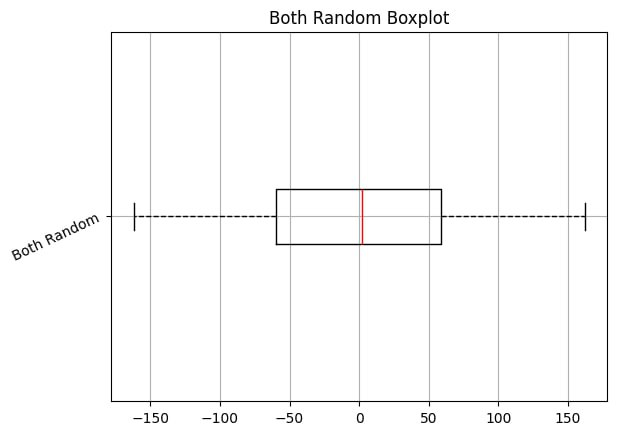
\includegraphics[scale=0.7]{RandomvsRandom.png}
\end{figure}\\
Here we can clearly see that our control simulation with RandomvsRandom has mean of approximately 0. \
Meaning that our sample size was sufficient enough to judge both agents as having the same performance.
\pagebreak
\subsection{Random Bot vs One Hand and Three Hand MiniMax}
One Hand MiniMax refers to MiniMax with Depth-Limit of 4, effectively making it maximize it's current score for one hand. 
The games were simulated wth 2 friendly players utilizing the MiniMax agent and the other 2 utilizing Random Agent.
\begin{figure}[h]
    \centering
    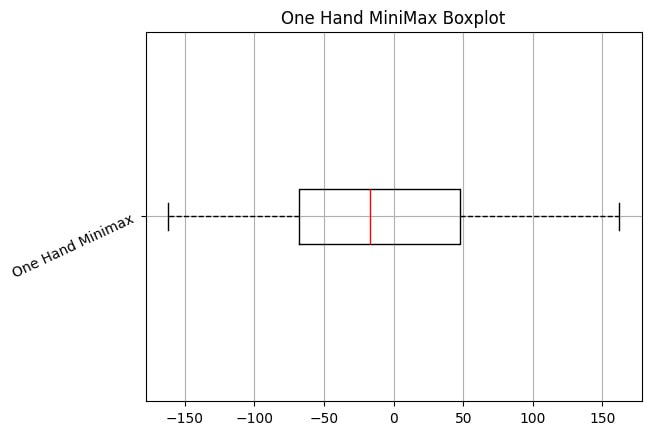
\includegraphics[scale=0.7]{OneHandMinimax.png}
\end{figure}\\
This graph shows the BoxPlot of points that each player gained after each round. 
Note that the point is not referring to the score that get's calculated based on gained points, but rather the actual added values of cards calculated after each hand.
We can see that One Hand MiniMax preformed worse than the Random Bot which was expected since in the game maximizing hands is not a good strategy. 
When a hand is maximized all of the trump cards are thrown in the beginning disregarding the potential to get more points by keeping them. 
\begin{figure}[h]
    \centering
    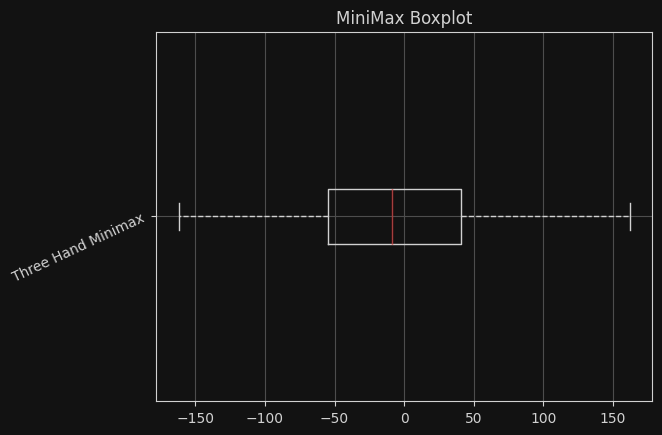
\includegraphics[scale=0.7]{ThreeHandMinimax.png}
\end{figure}\\
\pagebreak

In the Three hand version we can see that it is acting slightly better since in the last three hands it plays optimally since with the depth of 12 it can actually reach the terminal states.
However as was the case in the One Hand version it still lacks the ability to save trump cards in the beginning which over many games makes it on average worse than the Random Bot.
\begin{figure}[h]
    \centering
    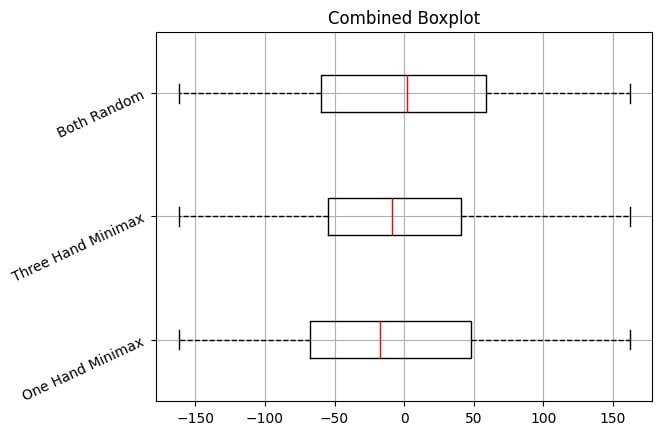
\includegraphics[scale=0.7]{Combined.png}
\end{figure}
\pagebreak

Here is the combined plot to better illustrate what we've discussed.
\pagebreak
\subsection{v1 Bidding Bot vs v1 Bidding Bot (Control)}
In order to understand the weakness of the first version of the Hill Climbing Agent(v1) we simulate about 500 games where the playing bots are all random and the bidding bots are both v1.
\begin{figure}[h]
    \centering
    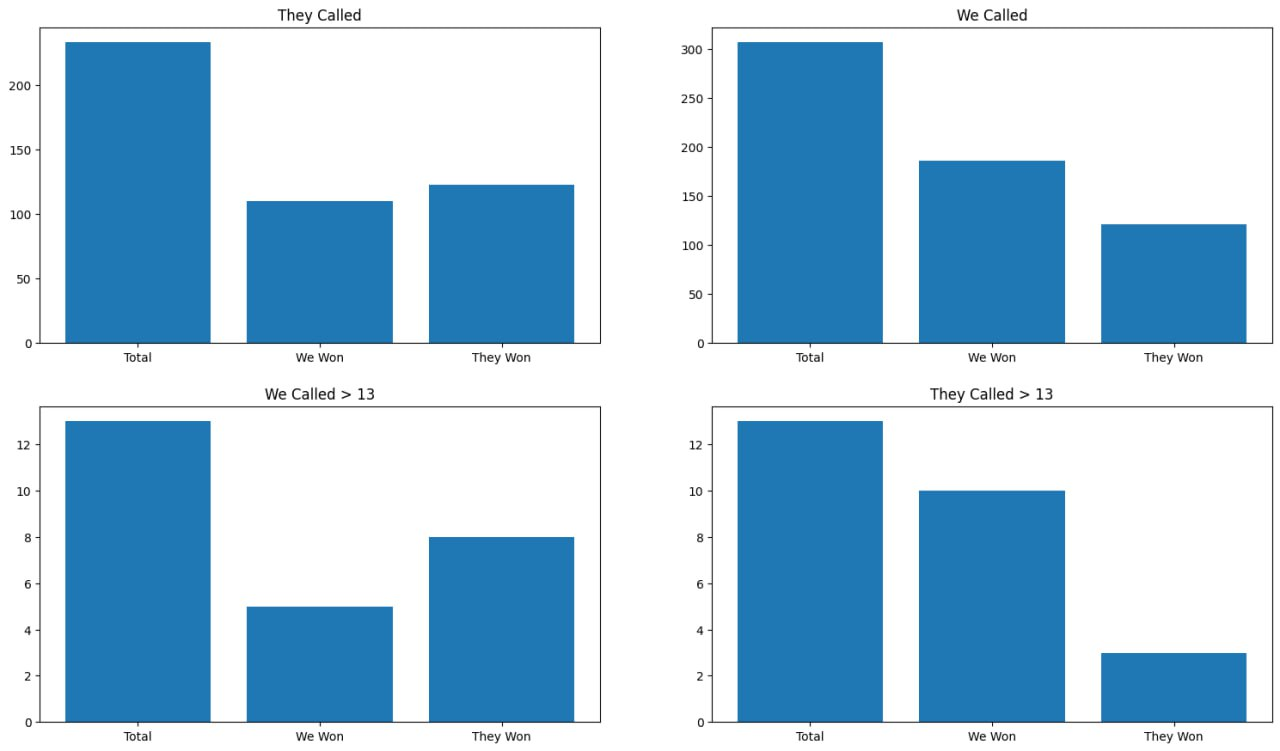
\includegraphics[scale=0.3]{Control.png}
\end{figure}\\
The top two graphs represent the rounds in which one side made the final bid and whether or not they won that round. 
From the graphs we can see that on average whoever calls wins more often than loses, but the problem that they overestimate how many points they can get is apparent. 
This is even more apparent in the bottom two graphs which are similar to the top two but are filtered to only shows when the bots made a big final bid.
In most of the cases when v1 makes a big final bid it loses the round which means we need to adjust the values to make it bid more realistically.
\pagebreak
\subsection{v1 Bidding Bot vs v2 Bidding Bot}
\begin{figure}[h]
    \centering
    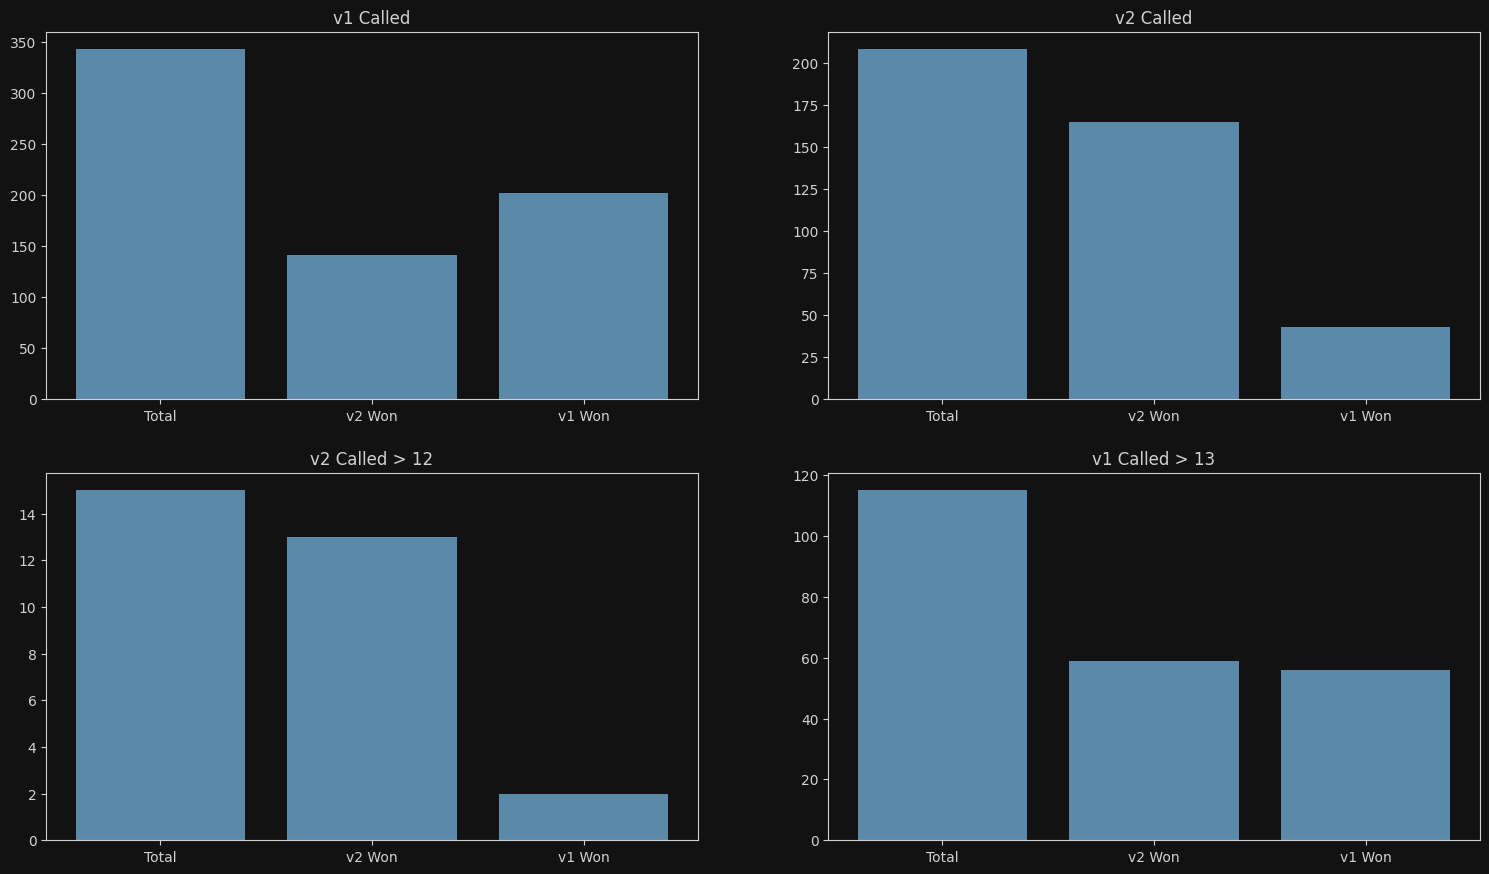
\includegraphics[scale=0.3]{V1vsV2.png}
\end{figure}
For our v2 of the Hill Climbing Algorithm with it's adjusted values we were able fix the problem of the v1 overestimating how many points it can get.
As we can see from the top two graphs when v1 makes the final bet it mostly wins, but with still many loses. 
In contrast when v2 makes the final bid it wins drastically more often. 
This is also apparent in the graphs where v2 makes a big final bid. By adjusting the confidence of the v1 we were
able to make it judge it's capacity to take points more accurately than before. 
